\subsection{Study design}
\label{sec:design}
\paragraph{Graphs.} Synthetic graphs (Erd\H{o}s--R\'enyi, stochastic block model with $20$ blocks and $10\%$ of edges between blocks, Barab\'asi--Albert, Watts--Strogatz with rewiring $0.1$; $n=2{,}000$, mean degree $10$) and two public graphs: the SNAP ego-Facebook graph (4,039 nodes; \citealt{mcauley2012learning}) and the Facebook100 Stanford3 graph (11,586 nodes, mean degree 98; \citealt{traud2012social,rossi2015network}; CC BY-SA). Both are anonymised structure only (ego-Facebook has no stated licence). Synthetic cells use 5 independent graph draws $\times$ 100 assignments, real graphs one graph $\times$ 500 assignments. Sweeps use a default SBM ($n=3{,}000$, mean degree 20) unless stated, with 8 graph draws $\times$ 250 assignments.
\paragraph{Mechanisms.} $Y_i=b_i+\mu_i(\bz)+\varepsilon_i$ with a fixed unit baseline $b_i$ (correlation $0.5$ with standardised log-degree plus an i.i.d.\ community component of SD $1$, so that position in the graph confounds the outcome) and Gaussian noise (SD $1$). M1: $\mu_i=\delta z_i+\gamma f_i$ (linear in the treated-neighbour fraction); M3: $\gamma g(f_i)$ with concave saturating $g(f)=(1-e^{-3f})/(1-e^{-3})$; M4: $\delta z_i+0.5f_i+0.5\,(W^2\bz)_i$ (one- plus two-hop interference); M5: M1 with $\gamma_i=\gamma(1+0.5\,s_i)$, $s_i$ the standardised log-degree. Defaults: $\delta=1$ and total spillover $1$ (interference-to-direct ratio $\rho=1$, so $\gate=2$ in all four). The main-grid parameters were fixed before any estimator results were seen; sweeps vary one factor at a time (Table~\ref{tab:setup} and Appendix).
\paragraph{Designs.} Bernoulli$(0.5)$, Bernoulli$(0.1)$, and graph-cluster randomisation (Louvain clusters, each cluster treated with probability $0.5$).
\paragraph{Estimators.} The difference in means (DM), a H\'ajek exposure estimator (strict full-neighbourhood exposure, with a $q=0.75$ variant for Bernoulli designs), and OLS on $(z,f)$ (\texttt{ols\_f}, the Chin-type estimator) with variants adding covariates, degree interactions, a two-hop feature or polynomial terms; ridge and gradient boosting appear in a smaller sub-experiment.
\paragraph{Metrics.} Bias, SD and RMSE of $\hat\gate-\gate$ over assignments, and RMSE and bias relative to $|\gate|$ (scale-free: ``fraction of the effect''). Also the coverage of nominal $95\%$ intervals (cluster-robust sandwich with Louvain communities as clusters, and a heteroskedasticity-robust one treating units as independent) and the share of replicates in which an estimator is undefined. Uncertainty: 95\% percentile bootstrap intervals over replicates for every plotted point; estimators share assignments and noise within a replicate (paired comparisons); an independent second seed set for the synthetic main grid is in Appendix~\ref{app:seed}.

\subsection{RQ1: how accurate is it?}
\begin{figure}[t]
\centering
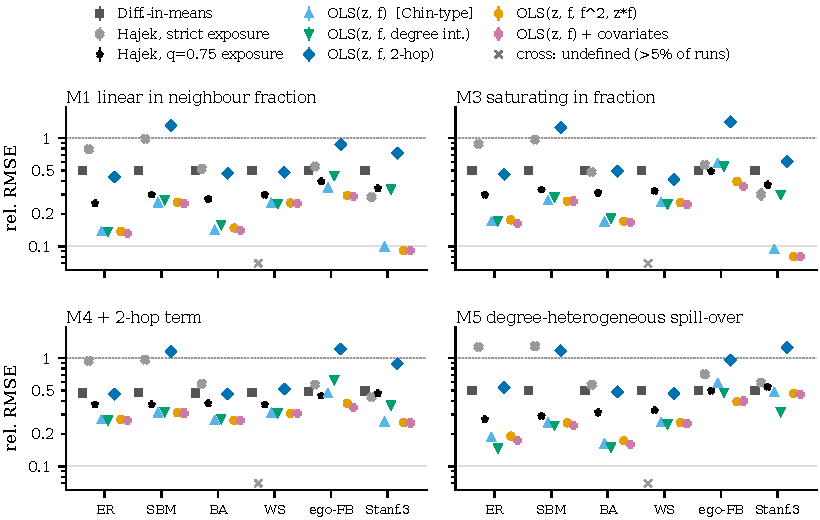
\includegraphics[width=0.99\linewidth]{fig1_headline.pdf}
\caption{Relative RMSE (RMSE$/|\gate|$, log scale, 95\% bootstrap CI) of each estimator on the 24 mechanism$\times$graph cells of the main grid under Bernoulli$(0.5)$, $\rho=1$. The difference in means has relative RMSE $\approx0.5$ everywhere because it recovers only the direct effect. Cells in which the strict H\'ajek estimator is undefined in more than 5\% of replicates are drawn as crosses. Other designs: Figures~\ref{fig:a1a}--\ref{fig:a1b}.}
\label{fig:headline}
\end{figure}
Figure~\ref{fig:headline} and Table~\ref{tab:failure} give the headline. Under Bernoulli$(0.5)$ with linear exposure (M1) the Chin-type OLS has median relative RMSE \MainOneOls{} across the six graphs against \MainDM{} for DM, and it is closer to the truth than DM in every graph of the main grid (Table~\ref{tab:failure}). Among the synthetic graphs, ER and BA (\MainOlsEr, \MainOlsBa) are easier than the SBM and Watts--Strogatz (\MainOlsSbm, \MainOlsWs); of the real graphs Stanford3 is easy (\MainStanOls) and ego-Facebook (\MainEgoOls) depends on the baseline draw (Fig.~\ref{fig:headline}; Sec.~\ref{sec:struct}). The strict H\'ajek estimator is no competitor under Bernoulli designs: it is undefined in a median of \HajekUndefBernLow{} of replicates at $p=0.1$, and at $p=0.5$ worse than OLS$(z,f)$ in every graph ($0.28$--$1.23$ against $0.10$--$0.34$). Adding a feature the mechanism does not need (the two-hop regressor under M1) is mainly a variance cost and is worse than DM on the SBM (\MainTwohopOneSbm), ego-Facebook (\MainTwohopOneEgo) and Stanford3 (\MainTwohopOneStan). The advantage is not uniform: under the saturating mechanism M3 at $p=0.1$ the Chin-type OLS has median relative RMSE \MainThreeBernLow{} and median relative bias \MainThreeBernLowBias{}, and it loses to DM on five of six graphs; only Stanford3, with its degree of 98, is better (Table~\ref{tab:failure}); two-hop interference (M4) gives a median relative bias of \MainFourBias{} at $p=0.5$, which a two-hop feature removes (\MainFourTwohopBias) at a variance price.

\begin{table}[t]
\centering\small
\caption{Main grid, median over six graphs [min, max] of relative RMSE of DM and of OLS$(z,f)$, median relative bias of OLS$(z,f)$, and the number of graphs on which OLS$(z,f)$ is better than / worse than / not significantly different from DM in paired MSE (95\% bootstrap CI of the MSE ratio, \texttt{results/contrasts.csv}).}
\label{tab:failure}
\begin{tabular}{@{}llccrc@{}}
\toprule
 & & \multicolumn{2}{c}{rel.\ RMSE, median [min, max]} & rel.\ bias & OLS better /\\
mech. & design & DM & OLS$(z,f)$ & OLS$(z,f)$ & worse / n.s.\ \\
\midrule
M1 & Bernoulli(0.5) & 0.50 [0.50, 0.50] & 0.19 [0.10, 0.34] & +0.00 & 6 / 0 / 0 \\
M1 & Bernoulli(0.1) & 0.50 [0.50, 0.51] & 0.31 [0.16, 0.57] & +0.00 & 5 / 1 / 0 \\
M1 & graph-cluster (p=0.5) & 0.27 [0.15, 0.37] & 0.18 [0.13, 0.25] & +0.00 & 4 / 1 / 1 \\
\addlinespace
M3 & Bernoulli(0.5) & 0.50 [0.50, 0.50] & 0.21 [0.09, 0.58] & -0.09 & 5 / 1 / 0 \\
M3 & Bernoulli(0.1) & 0.50 [0.50, 0.51] & 0.63 [0.30, 0.80] & +0.53 & 1 / 5 / 0 \\
M3 & graph-cluster (p=0.5) & 0.31 [0.18, 0.40] & 0.17 [0.16, 0.70] & -0.05 & 4 / 1 / 1 \\
\addlinespace
M4 & Bernoulli(0.5) & 0.48 [0.47, 0.49] & 0.29 [0.26, 0.47] & -0.22 & 5 / 0 / 1 \\
M4 & Bernoulli(0.1) & 0.48 [0.47, 0.50] & 0.38 [0.28, 0.63] & -0.21 & 5 / 1 / 0 \\
M4 & graph-cluster (p=0.5) & 0.33 [0.17, 0.40] & 0.22 [0.16, 0.59] & -0.06 & 3 / 2 / 1 \\
\addlinespace
M5 & Bernoulli(0.5) & 0.50 [0.50, 0.50] & 0.25 [0.16, 0.58] & -0.09 & 5 / 1 / 0 \\
M5 & Bernoulli(0.1) & 0.50 [0.50, 0.51] & 0.42 [0.23, 0.71] & -0.09 & 4 / 1 / 1 \\
M5 & graph-cluster (p=0.5) & 0.31 [0.17, 0.38] & 0.18 [0.16, 0.44] & -0.09 & 3 / 1 / 2 \\
\bottomrule
\end{tabular}

\end{table}

\subsection{RQ2: what determines the error?}
\paragraph{Variance dominates when the model is right, and is set by the design.}
Under correct specification the estimator is unbiased (|relative bias| $\le$ \EoneBiasMax{} for all $n$) and its SD falls as $n^{\EoneSlope}$ (fitted log--log slope; Fig.~\ref{fig:size}). Because DM has a constant bias of \EoneDMbias{} of the effect, OLS crosses it near $n=2{,}000$: at $n=500$ the regression is worse than DM (\EoneOLSA{} vs.\ \EoneDMA), at $n=8{,}000$ it is better (\EoneOLSC{} vs.\ \EoneDMC). The absolute SD of OLS is almost independent of the interference strength ($0.62$--$0.76$), so its error \emph{relative} to the effect $(1+\rho)$ falls with $\rho$ (Fig.~\ref{fig:gamma}); DM is much better with no interference ($\rho=0$: \EthreeDMZ{} vs.\ \EthreeOLSZ) and still better at $\rho=0.5$ (\EthreeDMH{} vs.\ \EthreeOLSH), and worse from $\rho=1$ (\EthreeDMO{} vs.\ \EthreeOLSO); at $\rho=4$ OLS has \EthreeOLSF{} against \EthreeDMF. Which graph quantities set the variance is predicted by P2: the SD grows with the (harmonic mean) degree, because the regressor $f$ then varies little across units and the coefficient of $f$ is weakly identified, and with the part of the baseline that is smooth over the graph. The predicted SD tracks the simulated one over \TheoryVarN{} graph draws (median ratio \TheoryVarMed, IQR \TheoryVarLo--\TheoryVarHi; Fig.~\ref{fig:theory}). Concretely, on the SBM the relative RMSE grows from \EtwoSbmLo{} at mean degree 5 to \EtwoSbmHi{} at 160, where DM would be better; on ER it grows more slowly (\EtwoErLo{} to \EtwoErHi, Fig.~\ref{fig:degree}). A community-level component of the baseline raises the error most: with $\sigma_c=0$ the relative RMSE is \EnineCzero{}, with $\sigma_c=3$ it is \EnineCthree{} (Fig.~\ref{fig:noise}), which is above DM's $0.5$.

\begin{figure}[t]
\centering
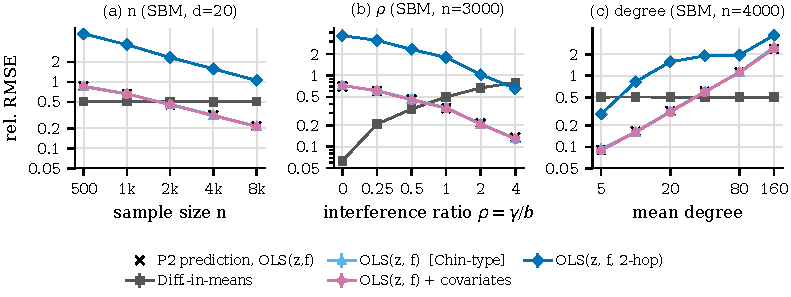
\includegraphics[width=0.96\linewidth]{figM_rmse_sweeps.pdf}
\caption{Relative RMSE of DM and OLS variants against (a) $n$ (SBM, mean degree 20), (b) the interference ratio $\rho$ ($n=3{,}000$) and (c) mean degree ($n=4{,}000$); 8 graph draws $\times$ 250 assignments per point. Crosses: closed-form P2 standard deviation of OLS$(z,f)$. Covariates change nothing visible; the two-hop regressor is worse except at $\rho=4$. Bias and SD panels, with the count-feature variants, are in Figs.~\ref{fig:sizeapp}--\ref{fig:gammaapp}.}
\label{fig:size}\label{fig:gamma}
\end{figure}

\paragraph{Bias comes from extrapolation and specification.}
The regression is fit where the exposure $f$ is concentrated near the design's $p$ and then evaluated at $f=0$ and $f=1$. P1 turns this into a computable asymptotic bias, $\beta_f^*-[g(1)-g(0)]$, which matches the noise-free population fits in \TheoryBiasN{} graph draws (correlation \TheoryBiasCorr, maximum absolute difference \TheoryBiasMaxDiff). Figure~\ref{fig:curv} shows what it implies: for each smooth response the bias vanishes at one value of $p$ and changes sign around it (for $f^{0.5}$ at degree 10 the relative bias is \EfourPowLo{} at $p=0.1$ and \EfourPowHi{} at $p=0.9$; for $f^2$ it is \EfourQuadMid{} at $p=0.5$ and \EfourQuadLo{}, \EfourQuadHi{} at $p=0.1,0.9$); for a threshold response at $f=0.5$ it is \EfourThrMidDten{} at $p=0.5$ and \EfourThrLoDten{}, \EfourThrHiDten{} at $p=0.1,0.9$. It is a population quantity, so more data do not reduce it, and higher degree does not either, since it concentrates $f$ around $p$: the threshold bias at $p=0.5$ grows from \EfourThrMidDten{} (degree 10) to \EfourThrMidDhund{} (degree 160). Whether a feature set can express the mechanism matters in the same way (Fig.~\ref{fig:spec}): adding a two-hop term to the signal gives a relative bias of \EsixTwohopBias{} for the Chin-type OLS on the SBM. The raw neighbour \emph{count} (scaled by mean degree) is confounded with degree and hence with the degree-correlated baseline: on ER with mean degree 60 its relative RMSE is \EsixCntErFrac{} when the truth is the fraction and \EsixCntEr{} when the truth is the count itself, and its relative bias is \EthreeCntZ{} even with no interference ($\rho=0$, Fig.~\ref{fig:gammaapp}). Controlling for log-degree and clustering removes this on ER (\EsixCntAdjErFrac{} and \EsixCntAdjEr), but on BA with fraction exposure the same adjusted regression has a relative bias of \EsixCntAdjBaBias{} (Fig.~\ref{fig:spec}). Heterogeneous spillovers that correlate with degree bias the estimator by P3 (M5 in Table~\ref{tab:failure}).
\begin{figure}[t]
\centering
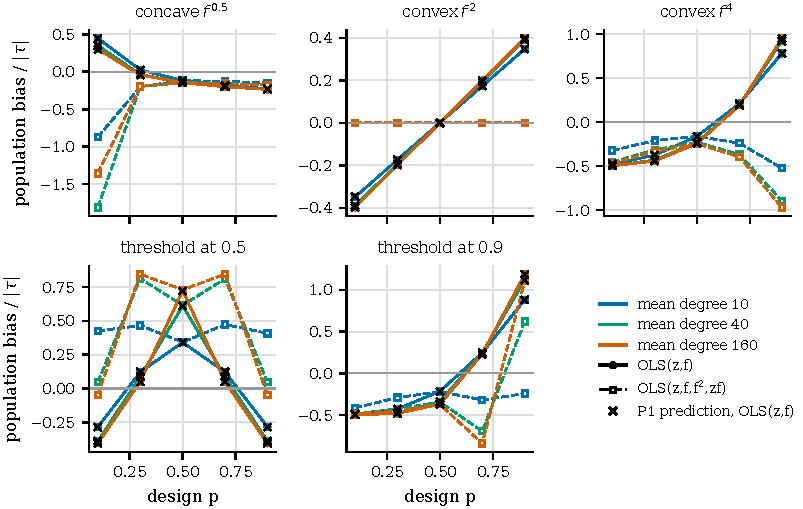
\includegraphics[width=0.97\linewidth]{fig8_curvature_population_bias.pdf}
\caption{Population (noise- and baseline-free) bias of OLS$(z,f)$ and of the quadratic OLS$(z,f,f^2,zf)$ relative to $|\gate|$, against the design $p$, for convex ($f^2$, $f^4$), concave ($f^{0.5}$) and threshold responses and mean degrees 10, 40, 160 (SBM, $n=3{,}000$). The estimand is exact; no sampling error enters. OLS$(z,f)$ is unbiased only at special $p$; the quadratic model removes the bias only when the truth is quadratic.}
\label{fig:curv}
\end{figure}

\paragraph{Flexible learners do not remove it.}
H2 predicted that tree ensembles, which do not extrapolate, would fail. The evidence is mixed (Fig.~\ref{fig:model}; fewer replicates: 4 graph draws $\times$ 80 assignments). Under linear exposure, ridge regression on rich features (relative RMSE \EsevenLinARidge{} at degree 10, \EsevenLinBRidge{} at degree 40) and a cubic OLS at degree 40 (\EsevenLinBCub) are far worse than OLS$(z,f)$ (\EsevenLinAOls, \EsevenLinBOls); boosting (\EsevenLinAGbm, \EsevenLinBGbm) is biased towards zero at degree 40 (relative bias \EsevenBiasLinBGbm). Under the threshold response OLS$(z,f)$ is biased (\EsevenBiasThrAOls{} and \EsevenBiasThrBOls{} at degrees 10 and 40), boosting is nearly unbiased (\EsevenBiasThrAGbm{}, \EsevenBiasThrBGbm) and has lower RMSE than OLS$(z,f)$ at degree 40 (\EsevenThrBGbm{} vs.\ \EsevenThrBOls) but not at degree 10 (\EsevenThrAGbm{} vs.\ \EsevenThrAOls); the cubic OLS is best at degree 10 (\EsevenThrACub) and worst at degree 40 (\EsevenThrBCub). No learner dominates; the bias--variance trade-off moves with the degree.
\begin{figure}[t]
\centering
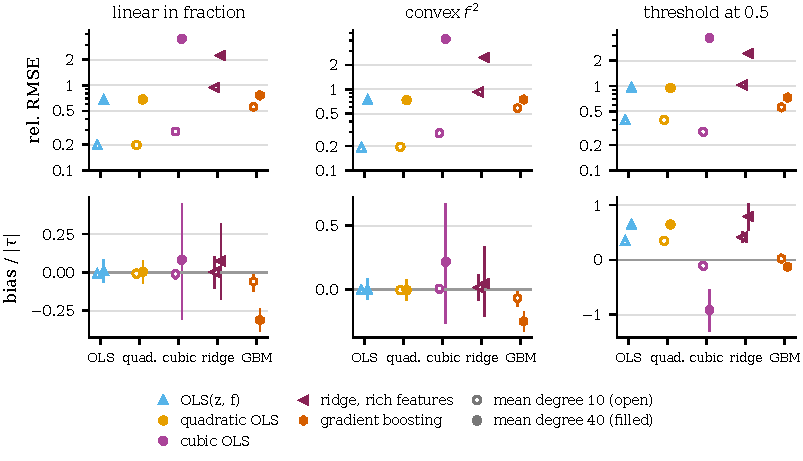
\includegraphics[width=0.97\linewidth]{fig15_model_class.pdf}
\caption{Model class (OLS, quadratic and cubic OLS, ridge on rich features, gradient boosting) under linear, convex and threshold exposure (SBM, $n=3{,}000$, $p=0.5$; open: mean degree 10, filled: 40). Relative RMSE and bias with bootstrap CIs; 4 graph draws $\times$ 80 assignments.}
\label{fig:model}
\end{figure}

\paragraph{A computable diagnostic works only for one family (negative result).}
H7 proposed that a data-computable exposure-support statistic, the distance (in SDs of the realised $f$) from the design's mean exposure to the farther of $f=0,1$, predicts the extrapolation error. Under Bernoulli designs it does for the saturating mechanism ($R^2=\HsevenSat$ in a log--log regression across cells) but not for power (\HsevenPow), threshold (\HsevenThresh), degree-heterogeneous (\HsevenHet) or two-hop (\HsevenBernTwohop) responses; pooled over all misspecified cells it explains $R^2=\HsevenPooled$ (\texttt{results/h7.csv}; Fig.~\ref{fig:h7} in the appendix shows the main grid). Within the ten cluster-randomised cells per mechanism the statistic is high for saturating (\HsevenClSat), two-hop (\HsevenClTwohop) and heterogeneous (\HsevenClHet) responses, but these are ten cells per mechanism that differ across graph families and not across $p$, so we do not weigh them against the Bernoulli result. We do not recommend the statistic as a general warning signal: it tells how far the extrapolation is, not whether the response is curved there.

\subsection{RQ3: where does it hold, where does it fail?}
\paragraph{Design.} Graph-cluster randomisation changes the conclusion: the median relative RMSE of DM falls from \MainDM{} to \MainDMClOne--\MainDMClFour{} across mechanisms (range $0.15$--$0.40$) because exposure is more often all-or-nothing, so the regression's advantage over DM under Bernoulli designs (\MainOneOls{} vs.\ \MainDM) largely disappears (Fig.~\ref{fig:design}); OLS is still better than DM in 14 of the 24 cluster-design graph--mechanism pairs (worse in 5, not distinguishable in 5; Table~\ref{tab:failure}), with OLS medians \MainOlsClThree--\MainOlsClFour{} against DM's. It also reduces extrapolation bias (M4: \MainFourBias{} $\to$ \MainFourBiasCl{} in Table~\ref{tab:failure}); for M3 the median OLS error under cluster randomisation (\MainOlsClThree) is close to that under the linear mechanism (\MainOlsClOne). A small $p$ is costly: variance rises as $1/\sqrt{p(1-p)}$ and nonlinear responses are extrapolated further (Table~\ref{tab:failure}, Bernoulli$(0.1)$ rows).

\paragraph{Network structure.}\label{sec:struct} OLS$(z,f)$ beats DM on \EfiveBetterN{} of ten graph families (relative RMSE \EfiveLo--\EfiveHi{} against DM's $0.5$) but not on ego-Facebook, where in this draw it is worse (\EfiveEgo; Fig.~\ref{fig:families}). The main grid and E5 use one draw of the synthetic baseline per real graph, and the same ego-Facebook specification gives a relative RMSE of \MainEgoOls{} in the main grid, \EelevenEgoZero{} in E11 and \EfiveEgo{} here, so we reran the 24 real-graph main cells with 8 independent baseline draws (60 assignments each). Under M1 and Bernoulli$(0.5)$ the relative RMSE of OLS$(z,f)$ on ego-Facebook has mean \RdEgoOneMean{} over the draws (range \RdEgoOneLo--\RdEgoOneHi, SD \RdEgoOneSd) against \RdEgoOneDM{} for DM, and on Stanford3 \RdStanOneMean{} (\RdStanOneLo--\RdStanOneHi). Over the four mechanisms at $p=0.5$ OLS beats DM in \RdStanWinsHalf{} of 32 draw--mechanism pairs on Stanford3 (\RdStanWinsTenth{} of 32 at $p=0.1$, \RdStanWinsCl{} under cluster randomisation) but in only \RdEgoWinsHalf{} of 32 on ego-Facebook (\RdEgoWinsTenth{} of 32 at $p=0.1$, \RdEgoWinsCl{} under cluster randomisation), with the saturating and degree-heterogeneous mechanisms the worst (\RdEgoThreeHalf{} and \RdEgoFiveHalf{} of 8). So Stanford3 favours regression robustly, whereas on ego-Facebook the answer depends on the baseline draw and DM is competitive; the count of families above is a single-draw count for ego-Facebook. Degree is the main structural driver (above); clustering and block structure matter through the baseline projection in P2 (at equal mean degree 20 and $n=4{,}000$ the relative RMSE is \EfiveEr{} on ER, \EfiveSbmMid{} on the SBM with $40\%$ of edges between blocks and \EfiveSbmLo{} with $2\%$; Fig.~\ref{fig:families}).

\paragraph{Graph errors.} Dropping and re-adding a share of edges when building the features biases the estimate towards zero, monotonically in the error rate, by $\EelevenSbmBias|\gate|$ at $50\%$ on the SBM and $\EelevenEgoBias|\gate|$ on ego-Facebook (Fig.~\ref{fig:grapherr}). At $\rho=1$ the relative RMSE rises from \EelevenSbmZero{} to \EelevenSbmGOne{} on the SBM (DM: \EelevenSbmGOneDM) and stays below DM, whereas on ego-Facebook it is already \EelevenEgoZero{} without errors and \EelevenEgoGOne{} at $50\%$ (about DM's level). With weak interference ($\rho=0.25$) the regression with an error-free graph already has relative RMSE \EelevenWeakOls{} against \EelevenWeakDM{} for DM, so DM wins at every error rate on both graphs.

\paragraph{Inference.} In the correctly specified linear mechanism the cluster-robust 95\% interval covers between \CovClMin{} and \CovClMax{} across graph families and sizes, below the nominal $95\%$ although the bias is negligible: on the SBM it improves with $n$ (\CovClSbmSmall{} at $n=1{,}000$ to \CovClSbmN{} at $4{,}000$), on BA it worsens (\CovClBaA{} to \CovClBaB). The interval that treats units as independent covers only \CovHcSbmLoA{} at $n=1{,}000$ and \CovHcSbmLoB{} at $4{,}000$ when baselines are community-structured and mixing is weak (\CovHcSbmMix{} and \CovHcSbmMixB{} for strong mixing), so its under-coverage grows with $n$; it covers $0.87$--$0.92$ on ER and BA (Fig.~\ref{fig:cover}). On the main grid coverage collapses once $|\text{bias}|/\mathrm{SD}>1$ (Fig.~\ref{fig:cov-bias}), as expected for an interval centred on a biased estimate. How coverage changes with $n$ when the model is misspecified (the second part of H6) was not tested.
\begin{figure}[t]
\centering
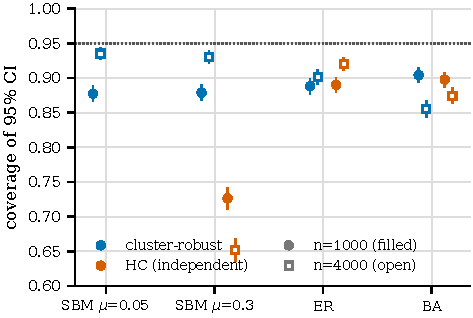
\includegraphics[width=0.57\linewidth]{fig13_coverage_n.pdf}
\caption{Coverage of the nominal 95\% interval for OLS$(z,f)$, cluster-robust versus independent-units standard errors, $n=1{,}000$ (filled) and $4{,}000$ (open), correct linear mechanism, 10 graph draws $\times$ 300 assignments.}
\label{fig:cover}
\end{figure}
